\section{Trådløs kommunikation via Bluetooth Low Energy}
\textit{Dette afsnit gennemgår design, implementering og test af systemets trådløse kommunikation mellem GAP peripheral og GAP central.}

\subsection{Design}
Systemet involverer to MCUer, henholdsvis en GAP central og en GAP peripheral. Begge enheder er påført et BLE modul, således dataoverførslen mellem enhederne foregår ved brug af dette. Denne dataoverførsel mellem MCUerne er illustreret på \figref{fig:blue_pseudo}. 
\begin{figure}[H]
	\centering
	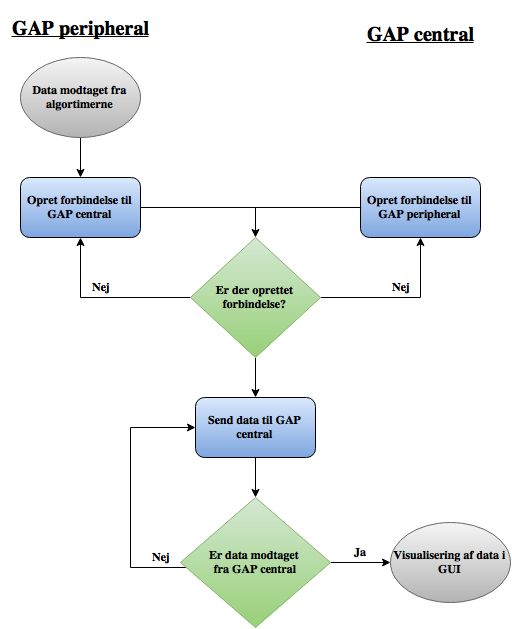
\includegraphics[scale=0.5]{figures/cDesign/blue_pseudo.png}
	\caption{På figuren ses flowchartet for den trådløse kommunikation og dataoverførsel mellem GAP central og peripheral.}
	\label{fig:blue_pseudo}
\end{figure}\vspace{-.25cm}
Der ses på \figref{fig:blue_pseudo} indledningsvist, at der forsøges at oprette forbindelse mellem enhederne, hvorefter dataoverførslen finder sted. Koden er bestemmende for, hvorvidt en MCU fungerer som GAP central eller peripheral i et kredsløb. Måden, hvorpå GAP central programmeres, er bestemmende for, om denne kan modtage data fra GAP peripheral. Ydermere skal GAP central overføre denne data til en computer gennem en USB pin, således visualisering i GUI er muligt. \newline
Førend dataoverførslen er mulig, skal der skabes en forbindelse mellem de to enheder, hvilket ligeledes fremgår af \figref{fig:blue_pseudo}. Hvis ikke dette lykkes, gentages proceduren indtil forbindelsen er oprettet. Systemet vil ikke fortsætte til næste element i algoritmen, medmindre dataoverførslen er fuldendt.  

\subsection{Implementering}
GAP peripheral er den MCU, der er ansvarlig for dataopsamling, signalbehandling og afsendelse af data til GAP central. Opsætningen af MCUerne som henholdsvis GAP central og peripheral udføres i PSoC Creator, hvor Topdesign af EZ-BLE modulerne er afgørende for rollen i kredsen. Standardkoder fra Cypress hjemmesider benyttes til indstilling af rollen for MCUen. \newline
4200M på GAP peripheral konfigureres således, at det færdigbehandlede data bliver ført mod EZ-BLE modulet. Denne konfiguration udføres ved at initialisere en UART forbindelse imellem de to mikroprocessorer samt indstille designet af pins i PSoC Creator.
Pin 3.0 på GAP peripheral 4200M benyttes til RX og pin~3.1 til TX. Ydermere konfigureres EZ-BLE modulet til at benytte pin~1.4 til RX og pin~1.5 til TX. Disse konfigurationer sikrer, at der forekommer en dataoverførsel fra 4200M og videre til EZ-BLE, hvorfra dataene kan sendes til GAP central via BLE.~\citep{Semiconductor20164200M} \newline
GAP central skal konfigureres således, at denne kan modtage data og herefter overføre dette til en computer gennem USB pinen. I denne konfiguration benyttes ligeledes til 4200M pin~3.0 til RX og pin~3.1 til TX og til EZ-BLE ligeledes pin~1.4 til RX og pin~1.5 til TX.

\subsection{Test}
BLE testes for at undersøge rækkevidden af denne kommunikation. Testen udføres på baggrund af de opstillede krav og tilhørende afvigelser opstillet i \secref{krav_BLE}. Kravene til den trådløse kommunikation er, at den trådløse kommunikation skal:
\begin{itemize}
	\item Være i stand til at sende data indenfor en rækkevidde på 2~meter. Der accepteres ikke en kortere rækkevidde.
\end{itemize}
I testen undersøges rækkevidden for den trådløse kommunikation ved, at GAP peripheral bliver sat til at videresende datapakker, som GAP central skal modtage. Hvis dataoverførslen er succesfuld, vil der ikke mangle nogle pakker. Dette bliver illustreret gennem MATLAB, hvori en succesfuld overførsel medfører en fuldstændig lineær kurve. Hvis datapakker er gået tabt, vil illustrationen af antal modtagne pakker variere fra antal sendte pakker med stor hældning, og kurven vil ikke være lineær. Denne test udføres med forøget afstand mellem GAP peripheral og central, hvoraf den maksimale afstand for succesfuld dataoverførsel kommer til udtryk. \\
Datapakkerne i denne test sendes fire gange i sekundet, og resultaterne bliver opsamlet over 30~sekunder. Der skabes forbindelse mellem GAP peripheral og central, hvor antallet af modtagne datapakker optages af Realterm. Derfra konverteres det fra hex til decimaltal, hvormed data kan plottes i MATLAB.\fxnote{capture, optaget i hex, konverteret til decimaltal, som er plottet i matlab}
\begin{table}[H]
	\centering
	\begin{tabular}{cc}
			\hline
		\rowcolor[HTML]{C0C0C0} 
		Afstand {[}m{]} & Tabte datapakker \\ 	\hline
		0,5 	& 0\% \\ 	\hline
		1,0		& 0\% \\	\hline
		1,5 	& 0\% \\	\hline
		2,0		& 0\% \\	\hline
		2,5 	& 0\% \\	\hline
		3,0		& 0\% \\	\hline
		3,5 	& 0\% \\	\hline
		4,0		& 100\% \\	\hline
	\end{tabular}
	\caption{I tabellen ses sammenhængen mellem antal tabte datapakker omregnet til procent og afstanden mellem GAP peripheral og central.}
	\label{test:ble_overforsel}
\end{table}\vspace{-.25cm}
Testresultaterne i \tabref{test:ble_overforsel} viser, at med en afstand på mere end 3,5~meter kan GAP peripheral og central ikke opretholde forbindelsen. Dette fremgår ligeledes af \figref{fig:test_ble}, hvor der ses, at antallet af sendte og modtagende pakker har en lineær sammenhæng op til 3,5~meter.
\begin{figure}[H]
	\centering
	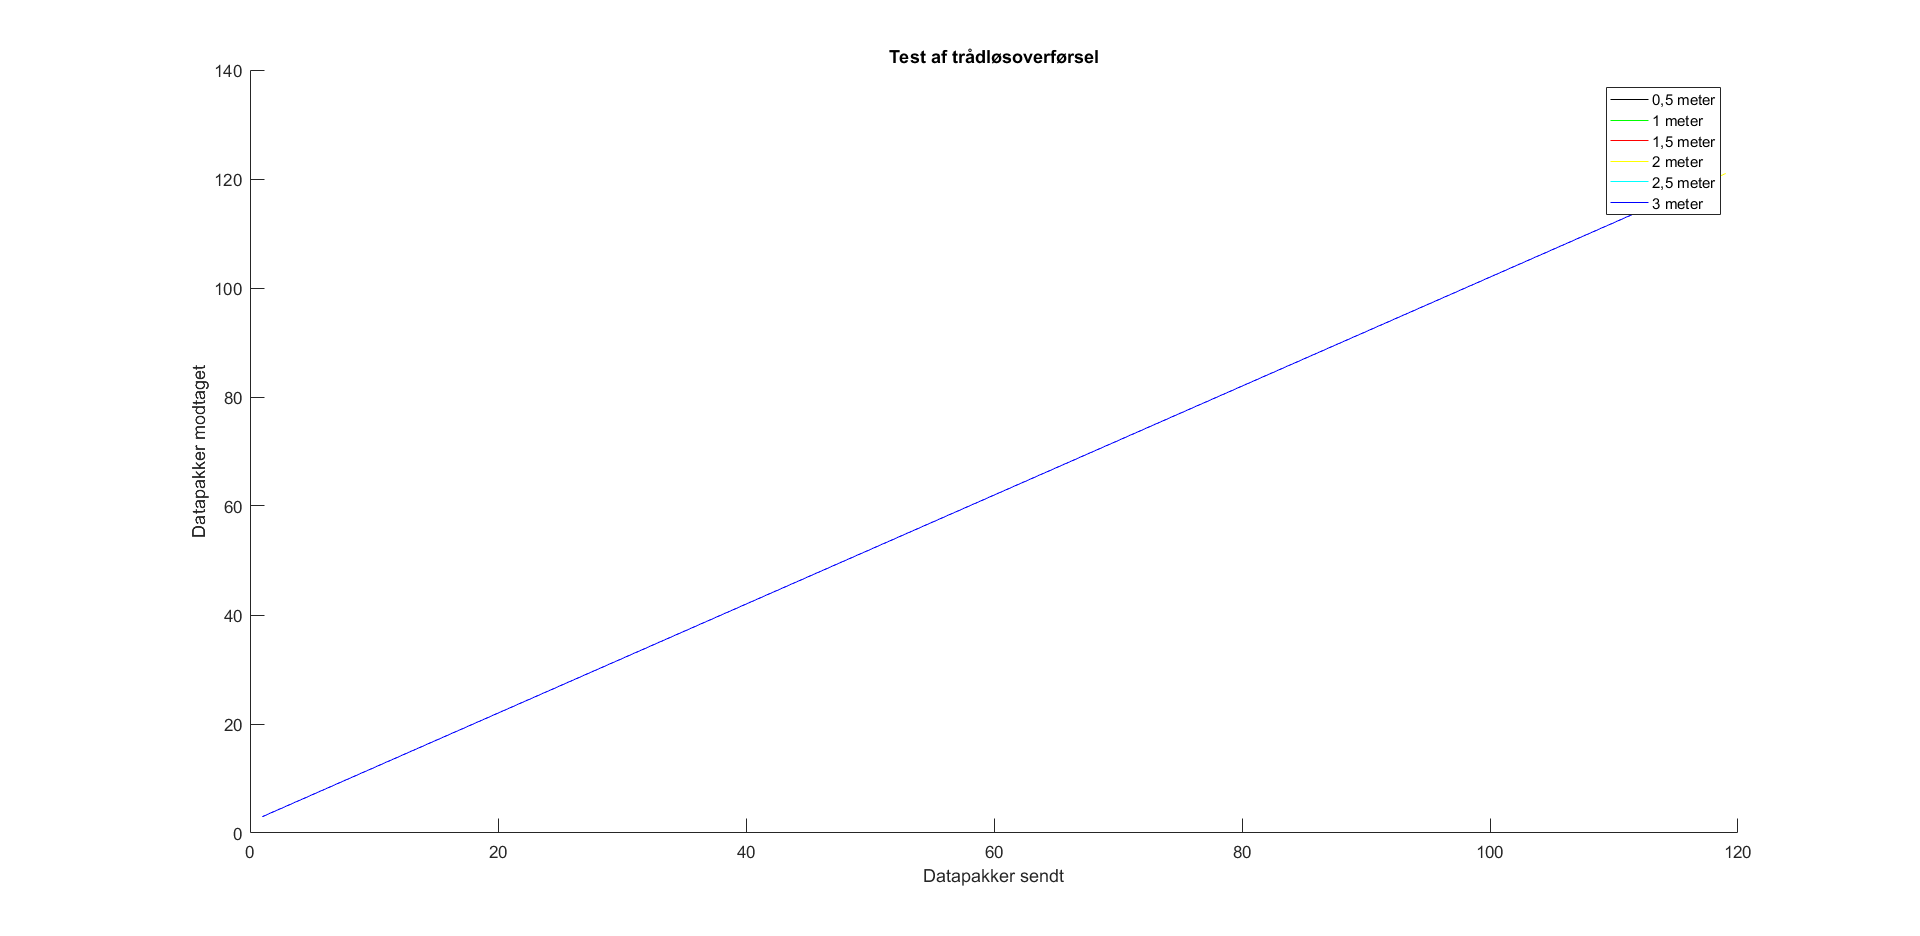
\includegraphics[scale=0.35]{figures/cDesign/test_ble.png}
	\caption{På figuren ses et grafisk plot af forholdet mellem antal sendte pakker sammenholdt med antal modtagne datapakker. }
	\label{fig:test_ble}
\end{figure}\vspace{-.25cm}
Alle datapakker op til 3,5~meter bliver modtaget, hvorfor der ikke forekommer udsalg på \figref{fig:test_ble}. På figuren ses den blå kurve, da alle kurver til med og 3,5 plottes oveni hinanden. Derudover ses det, at den røde kurve for 4~meter har en værdi af 0, da ingen pakker modtages ved denne afstand. \\
Kravet om, at data mellem de to MCUer udelukkende skal sendes med trådløs kommunikation i form af BLE, er dermed muligt at opfylde. Den trådløse kommunikation mellem systemets enheder overholder kravet vedrørende afsendelse og modtagelse af data inden for 3~meters afstand. Kravet vedrørende tab af data heraf overholdes ligeledes, da datapakker først går tabt over 3,5~meters afstand.
